\documentclass{beamer}
\usepackage{booktabs,tikz,float}
\renewcommand{\arraystretch}{1.25}
%\usetheme{Berlin}
\title{Diversification}
\newcommand{\fttheory}[1]{\fcolorbox{blue}{blue}{\color{white}\textbf{#1}\hspace{\textwidth}}}
\newcommand{\ftexampl}[1]{\fcolorbox{orange}{orange}{\color{black}\textbf{#1}\hspace{\textwidth}}}
\newcommand{\ftdata}[1]{\fcolorbox{violet}{violet}{\color{white}\textbf{#1}\hspace{\textwidth}}}
\newcommand{\ftheader}[1]{\fcolorbox{lightgray}{lightgray}{\color{black}\textbf{#1}\hspace{\textwidth}}}
\begin{document}
%\maketitle

\begin{frame}{\ftheader{Introduction: Diversification}}
	\begin{itemize}
		\item In this lecture, we begin our study of portfolio design
		\item In order to properly design portfolios, we need to understand how the returns of the stocks in the portfolio co-move (covary, correlate, etc.)
		\item We will learn that by choosing stocks that do not co-move too much, we can lower the risk of the portfolio without sacrificing return
		\item This is known as diversification
		\item We will introduce diversification with three stylized examples
	\end{itemize}
\end{frame}

\begin{frame}{\ftexampl{Example 1}}
	Suppose that $R_{F}=0$. Consider two stocks, $A$ and $B$: 
	\begin{table}[H]
		\begin{center}
			\begin{tabular}{crrr}
				Stock & $E[R]$ & $SD[R]$ & $SR[R]$ \\ \hline 
				$A$ & 5\% & 20\% & 0.25 \\  
				$B$ & 4\% & 20\% & 0.20
			\end{tabular}
		\end{center}
	\end{table} 
	Stock $B$'s Sharpe ratio is smaller than that of stock $A$. Why would anyone \underline{ever} buy stock $B$?
\end{frame}

\begin{frame}{\ftexampl{Example 1}}
	Suppose that $A$ and $B$ have a correlation of $0.5$. Then
	\begin{align*}
		\text{Var}[R_{P}]&=x_{A}^{2}\text{SD}[R_{A}]^{2}+x_{B}^{2}\text{SD}[R_{B}]^{2}+2x_{A}x_{B}\text{Cov}[R_{A},R_{B}]\\
		&=x_{A}^{2}\text{SD}[R_{A}]^{2}+x_{B}^{2}\text{SD}[R_{B}]^{2}\\
		&\hspace{.5in}+2x_{A}x_{B}\text{SD}[R_{A}]\text{SD}[R_{B}]\text{Corr}[R_{A},R_{B}]\\
		&=(.5)^2(.2)^2+(.5)^2(.2)^2+2(.5)(.5)(.2)(.2)(.5)\\
		&=.03
	\end{align*}
	and hence $\text{SD}[R_{P}]=17.3205\%$. 
\end{frame}

\begin{frame}{\ftexampl{Example 1}}
	Take a portfolio-based perspective:
	\begin{table}[H]
		\begin{center}
			\begin{tabular}{rrrrr}
				$x_{A}$ & $x_{B}$ & $E[R]$ & $SD[R]$ & $SR[R]$ \\ \hline 
				100\% & 0\% & 5\% & 20\% & 0.25 \\  
				0\% & 100\% & 4\% & 20\% & 0.20\\ \hline
				50\% & 50\% & 4.5\% & 17.3205\% & 0.2598
			\end{tabular}
		\end{center}
	\end{table} 
	The new portfolio returns less than stock $A$ on average (4.5\% instead of 5\%), but has less volatility (17.3205\% instead of 20\%).\\
	\vfill
 	\noindent\textbf{Moral:} a low-Sharpe ratio stock can increase the portfolio-Sharpe ratio above the Sharpe ratios of any of the constituent stocks
\end{frame}

\begin{frame}{\ftexampl{Example 2}}
	Suppose that $R_{F}=0$. Consider three stocks: $A$, $B$, and $C$. For each stock, $E[R]=5\%$ and $SD[R]=20\%$. Therefore, all stocks have a Sharpe ratio of 0.25. The correlations are 
	\begin{align*}
		\text{Corr}[R_{A},R_{B}]&=0.75\\
		\text{Corr}[R_{B},R_{C}]&=0.50\\
		\text{Corr}[R_{A},R_{C}]&=0.25
	\end{align*}
	Suppose you can only pick two of the three stocks. Which pair would you choose? Suppose that you invest equally in the two stocks. 
\end{frame}

\begin{frame}{\ftexampl{Example 2}}
	Let's compute the Sharpe ratios of each of the three portfolios.
	\begin{table}[H]
		\begin{center}
			\begin{tabular}{rrr|r|rrr}
				$x_{A}$ & $x_{B}$ & $x_{C}$ & \text{Corr} & $\text{E}[R]$ & $\text{SD}[R]$ & $\text{SR}[R]$ \\ \hline 
				50\% & 50\% & 0\% & 0.75 & 5\% & 18.7083\% & 0.2673\\  
				0\% & 50\% & 50\% & 0.50 & 5\% & 17.3205\% & 0.2887 \\
				50\% & 0\% & 50\% & 0.25 & 5\% & 15.8114\% & 0.3162
			\end{tabular}
		\end{center}
	\end{table} 
	We should choose the portfolio with stocks $A$ and $C$.\\
	\vfill
 	\noindent\textbf{Moral:} By choosing less correlated stocks, we can increase the portfolio-Sharpe ratio \underline{without} sacrificing return.
\end{frame}

\begin{frame}{\ftexampl{Example 3}}
	Suppose that $R_{F}=0$. Consider three stocks: $A$, $B$, and $C$. For each stock, $E[R]=5\%$ and $SD[R]=20\%$. Therefore, all stocks have a Sharpe ratio of 0.25. The correlations are 
	\begin{align*}
		\text{Corr}[R_{A},R_{B}]&=+1\\
		\text{Corr}[R_{A},R_{C}]&=-1
	\end{align*}
	What are the expected returns, volatilities, and Sharpe ratios of each of the pairs?
\end{frame}

\begin{frame}{\ftexampl{Example 3}}
	Let's compute the Sharpe ratios of each of the three portfolios.
	\begin{table}[H]
		\begin{center}
			\begin{tabular}{rrr|r|rrr}
				$x_{A}$ & $x_{B}$ & $x_{C}$ & \text{Corr} & $\text{E}[R]$ & $\text{SD}[R]$ & $\text{SR}[R]$ \\ \hline 
				50\% & 50\% & 0\% & $+1$ & 5\% & 20\% & .25\\  
				50\% & 0\% & 50\% & $-1$ & 5\% & 0\% & ?
			\end{tabular}
		\end{center}
	\end{table} 
	We should choose the portfolio with stocks $A$ and $C$. This portfolio is perfectly hedged. It is equivalent to a risk-free asset.\\
	\vfill
	\noindent\textbf{Moral:} Perfectly positively correlated stocks behave like one stock, while perfectly negatively correlated stocks behave like the risk-free asset
\end{frame}

\begin{frame}{\fttheory{Risk-Return Space}}
	\begin{itemize}
		\item Let's look at Apple (AAPL) and Proctor \& Gamble (PG)
		\item Their returns have a correlation of 0.3162
	\end{itemize}
	\begin{table}[H]
		\begin{center}
			\begin{tabular}{lrrr}
				Stock & $E[R]$ & $SD[R]$ & $SR[R]$ \\ \hline 
				AAPL & 2.24\% & 7.47\% & 0.3133\\  
				PG & 0.93\% & 3.86\% & 0.2409
			\end{tabular}
		\end{center}
	\end{table} 
	\begin{itemize}
		\item Let's plot this information in risk-return space
	\end{itemize}
\end{frame}

\begin{frame}{\fttheory{Risk-Return Space}}
	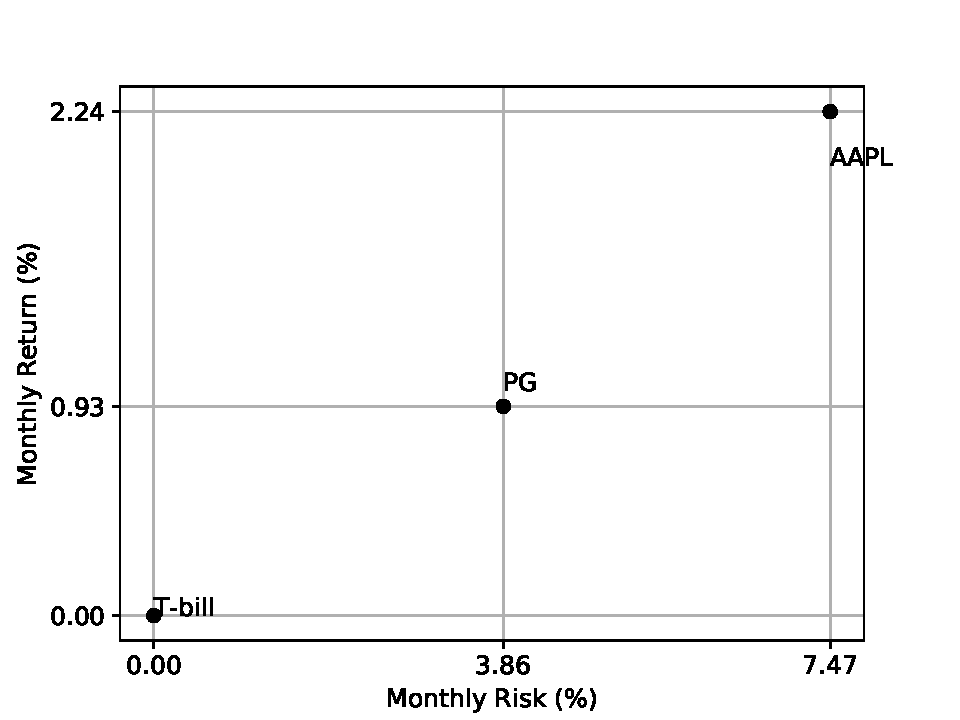
\includegraphics[scale=.65]{blank}
\end{frame}

\begin{frame}{\fttheory{Risk-Return Space: Efficient Frontier}}
	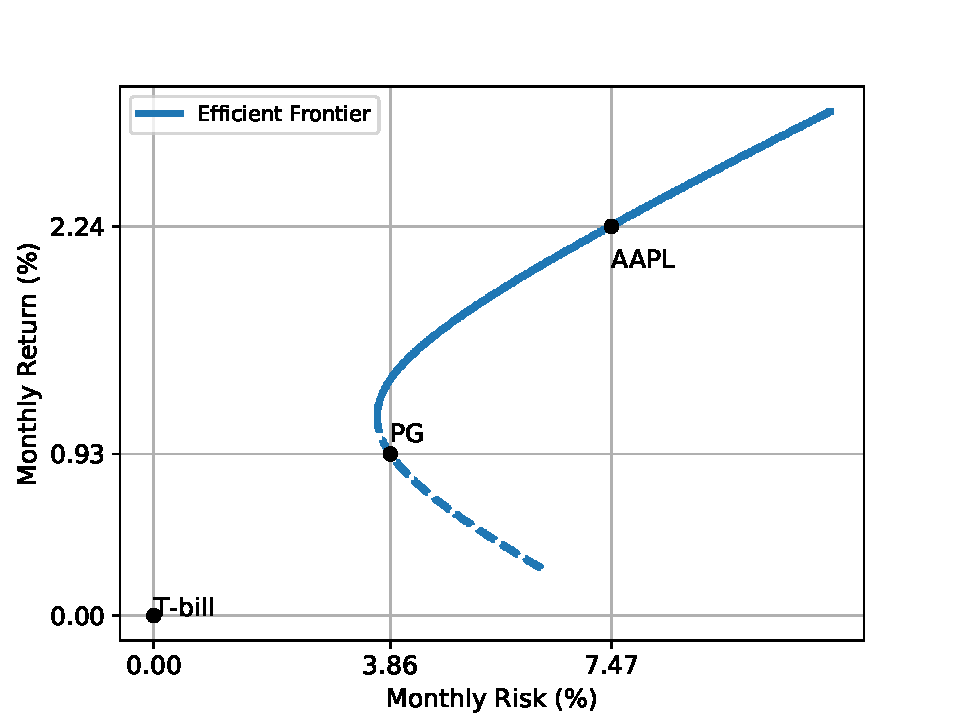
\includegraphics[scale=.65]{frontier}
\end{frame}

\begin{frame}{\fttheory{Risk-Return Space: Efficient Frontier}}
	\begin{itemize}
		\item For two stocks, the efficient frontier is the graph of the risks and returns of each portfolio containing the two stocks
		\item For example, a portfolio that is 100\% in Apple and 0\% in P\&G corresponds to the point labelled AAPL; a portfolio that is 0\% in Apple and 110\% in P\&G corresponds to the point labelled PG; a portfolio that is 50\% in Apple and 50\% in P\&G corresponds to a point along the blue line between AAPL and PG; a portfolio that is 150\% in Apple and -50\% in P\&G corresponds to a point along the blue line north-east of AAPL
		\item Portfolios associated with points along the dashed line are inefficient, in the sense that for each such portfolio (associated with a point on the bottom of the graph), one can find a portfolio with the same risk but a higher return (associated with a point on the top of the graph)
	\end{itemize}
\end{frame}

\begin{frame}{\ftexampl{Example 4}}
	Suppose you construct a portfolio that is $+150\%$ in AAPL and $-50\%$ in PG. Discuss the sequence of cash flows when you initiate the position. \\
	\pause
	{\color{blue}
		Suppose you have 10k USD of capital. Short PG. You collect 5k USD. Together with your 10k USD, buy 15k of AAPL. 
	}
\end{frame}

\begin{frame}{\fttheory{Risk-Return Space: Capital Allocation Line (CAL)}}
	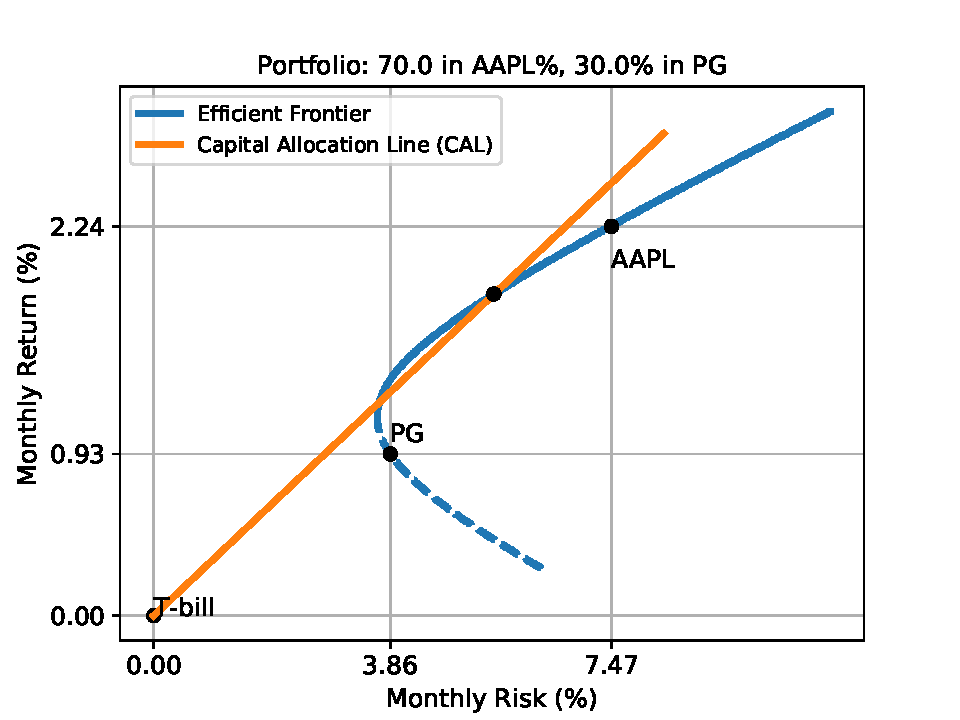
\includegraphics[scale=.65]{big_aapl}
\end{frame}

\begin{frame}{\fttheory{Risk-Return Space: Capital Allocation Line (CAL)}}
	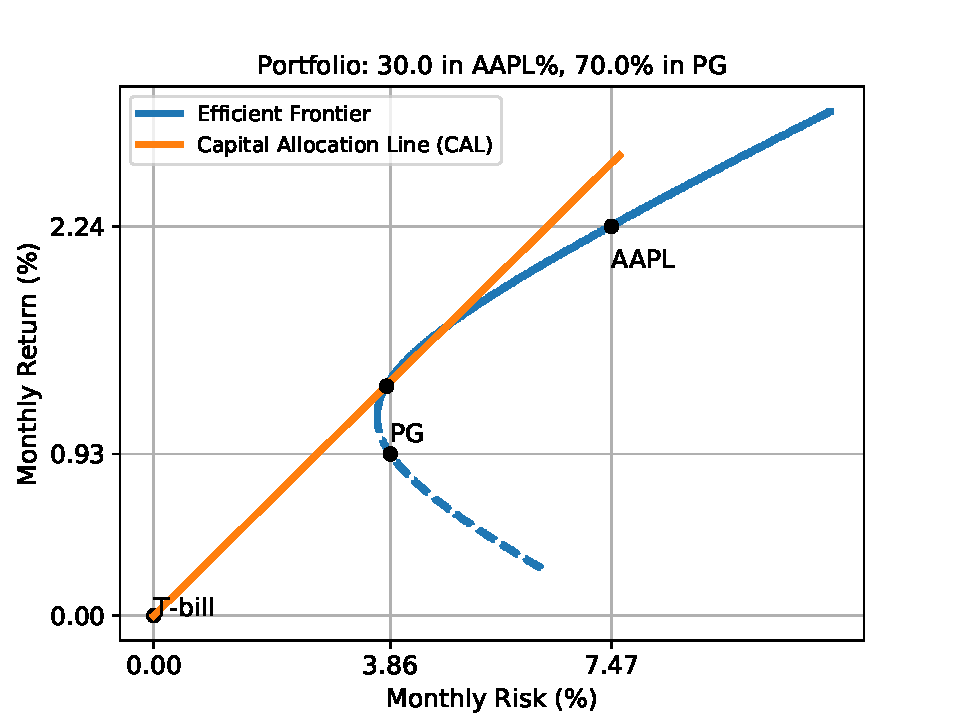
\includegraphics[scale=.65]{big_pg}
\end{frame}

\begin{frame}{\fttheory{Risk-Return Space: Tangency Portfolio}}
	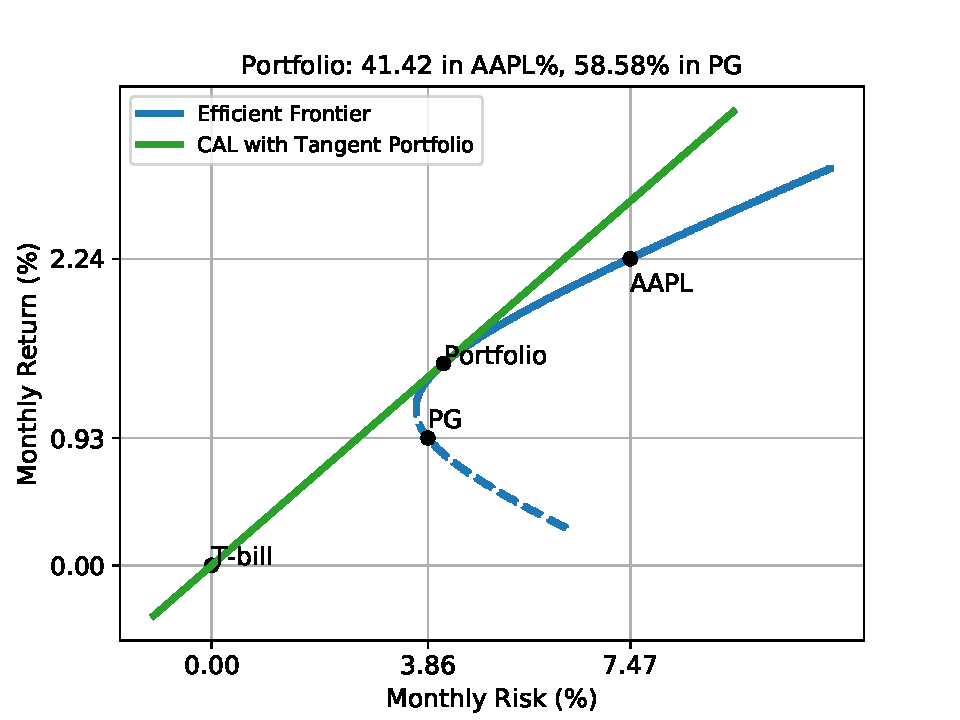
\includegraphics[scale=.65]{tangency}
\end{frame}

\begin{frame}{\fttheory{Risk-Return Space: Capital Allocation Line (CAL)}}
	\begin{itemize}
		\item The Capital Allocation Line (CAL) consists of the risks and returns of each portfolio containing the risk-free asset and (a portfolio of) the two stocks
		\item We can construct CALs for any portfolio: we have constructed CALs (the orange lines) for portfolios that are 70\% in Apple, 30\% in P\&G; 70\% in Apple, 30\% in P\&G)
		\item By pushing the CAL as far north-west as we can while still intersecting the risk-free asset and the efficient frontier, we obtain the tangency portfolio and its CAL (the green line)
		\item It so happens that this portfolio is 41.42\% in Apple and 58.58\% in P\&G
	\end{itemize}
\end{frame}

\begin{frame}{\fttheory{Tangency Portfolio}}
	\begin{itemize}
		\item Among all CALs, the one that includes the tangency portfolio has the highest Sharpe Ratio 
		\item To compute the weights of the tangency portfolio, define
		\begin{align*}
			\widetilde{x}_{A}&=\text{SD}[R_{B}](\text{SR}[R_{A}]-\text{SR}[R_{B}]\text{Corr}[R_{A},R_{B}])\\
			\widetilde{x}_{B}&=\text{SD}[R_{A}](\text{SR}[R_{B}]-\text{SR}[R_{A}]\text{Corr}[R_{A},R_{B}])
		\end{align*}
		The weights of the tangency portfolio are
		\begin{align*}
			x_{A}&=\frac{\widetilde{x}_{A}}{\widetilde{x}_{A}+\widetilde{x}_{B}}\\
			x_{B}&=\frac{\widetilde{x}_{B}}{\widetilde{x}_{A}+\widetilde{x}_{B}}
		\end{align*}
	\end{itemize}
\end{frame}

\begin{frame}{\ftheader{Many Stocks}}
	\begin{itemize}
		\item Thus far, we have studied portfolios consisting of two stocks
		\item What about portfolios consisting of more than two stocks?
		\item Consider $N\geq2$ stocks, $1,2,\ldots,N$
		\item The general problem is to choose weights $x_{1},x_{2},\ldots,x_{N}$ to minimize the portfolio variance
		\begin{equation}
			\text{Var}[R_{P}]=\text{Var}[x_{1}R_{1}+x_{2}R_{2}+\cdots+x_{N}R_{N}]
		\end{equation}
		given an expected return $\mu$
		\begin{equation}
			\mu=\text{E}[R_{P}]=\text{E}[x_{1}R_{1}+x_{2}R_{2}+\cdots+x_{N}R_{N}]
		\end{equation}
		and $x_{1}+x_{2}+\cdots+x_{N}=1$
		\item One can solve this problem using \textit{quadratic programming}
	\end{itemize}
\end{frame}

\begin{frame}{\ftdata{Correlations}}
	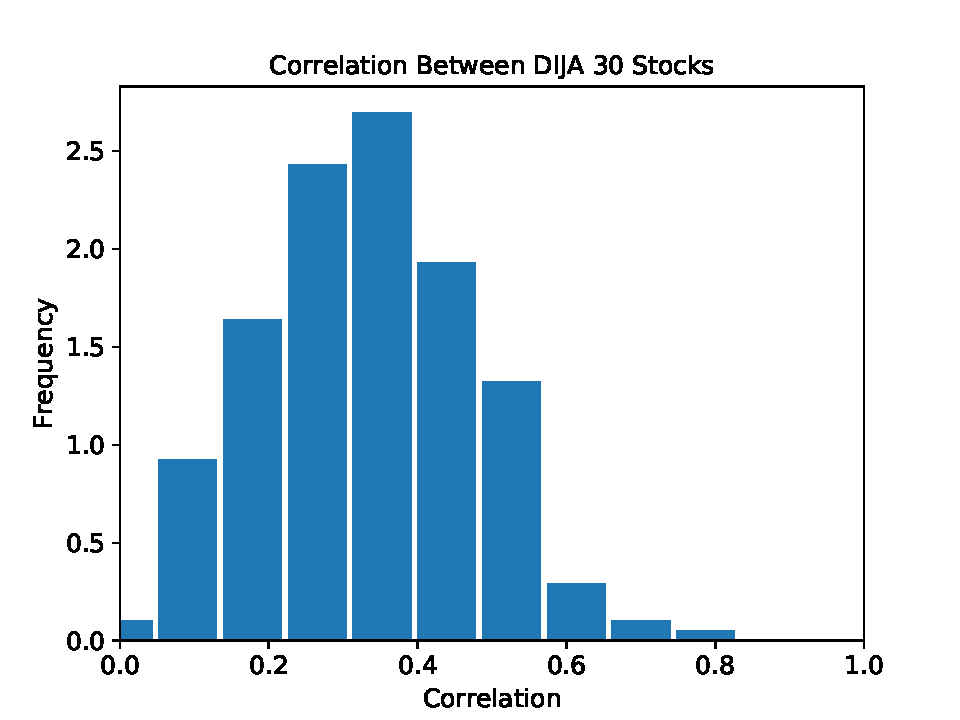
\includegraphics[scale=.7]{correlations}
\end{frame}

\begin{frame}{\fttheory{Special Cases}}
	\begin{enumerate}
		\item If the stocks are uncorrelated, the portfolio has mean and variance
			\begin{align}
				\text{E}[R_{P}]&=x_{1}\text{E}[R_{1}]+x_{2}\text{E}[R_{2}]+\cdots+x_{N}\text{E}[R_{N}]\\
				\text{Var}[R_{P}]&=x_{1}^{2}\text{Var}[R_{1}]+x_{2}^{2}\text{Var}[R_{2}]+\cdots+x_{N}^{2}\text{Var}[R_{N}]
			\end{align}
		\item An equally weighted portfolio of $N$ independent, identically distributed stocks with mean $\mu$, variance $\sigma^{2}$, and correlation $\rho$ has mean and variance
			\begin{align}
				\text{E}[R_{P}]&=\mu\\
				\text{Var}[R_{P}]&=\sigma^{2}\left(\frac{1}{N}+\left(1-\frac{1}{N}\right)\rho\right)
			\end{align}
			Note that $\text{Var}[R_{P}]\rightarrow\rho\sigma^{2}$ as $N\rightarrow\infty$
	\end{enumerate}
\end{frame}

\begin{frame}{\ftexampl{Example 5}}
	The average standard deviation and correlation of stocks in the Dow Jones Industrial Average are 5.72\% and 0.33 respectively. What is the standard deviation of an equally-weighted portfolio of 2 stocks? 4 stocks? 8 stocks?\\
	\pause	
	{\color{blue}
	\begin{align*}
		\text{SD}[R_{\text{2 Stocks}}]&=\sqrt{(.0572)^{2}\left(\frac{1}{2}+\left(1-\frac{1}{2}\right)(0.33)\right)}=4.6645\%\\
		\text{SD}[R_{\text{4 Stocks}}]&=\sqrt{(.0572)^{2}\left(\frac{1}{4}+\left(1-\frac{1}{4}\right)(0.33)\right)}=4.0345\%\\
		\text{SD}[R_{\text{8 Stocks}}]&=\sqrt{(.0572)^{2}\left(\frac{1}{8}+\left(1-\frac{1}{8}\right)(0.33)\right)}=3.6793\%
	\end{align*}
	}
\end{frame}

\begin{frame}{\ftdata{The Value of Diversification}}
	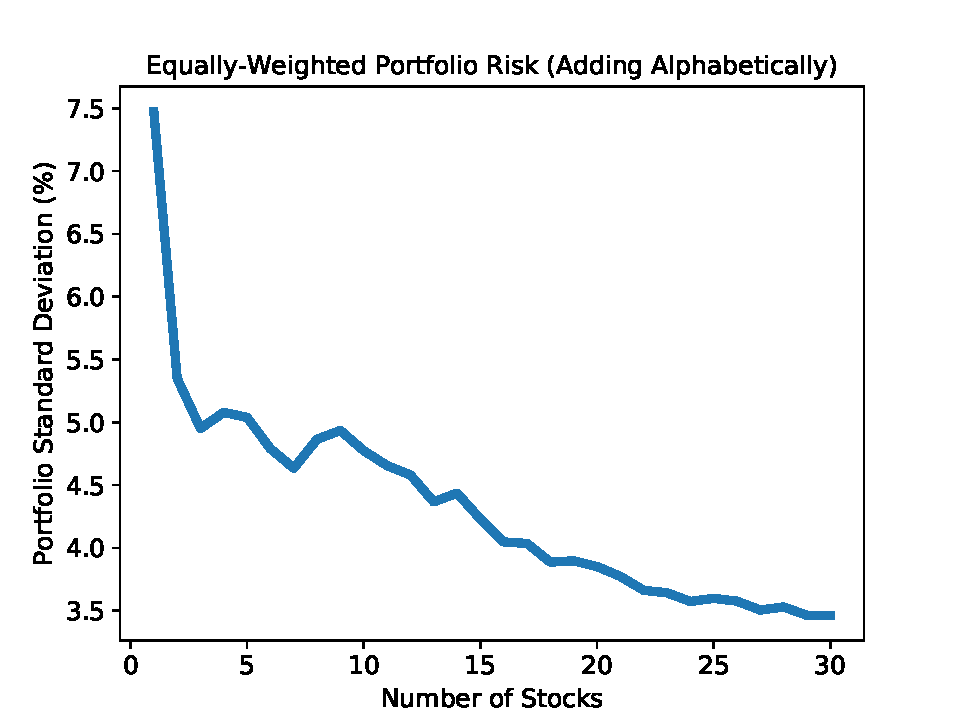
\includegraphics[scale=.7]{div30}
\end{frame}

\iffalse
\begin{frame}{\ftexampl{Example 6}}
	According to the Social Security Administration, the distribution of womens' lifespans has a mean 80.93 years and a standard deviation of 14.46 years. Let's round to 81 and 14 years respectively. Suppose you start a life insurance company that sells 100k USD life insurance policies to 40-year-old women (and suppose further that deaths in you pool are uncorrelated). Computing the present-value of 100k USD at 1.5\% for $0,1,2,\ldots$ years until death, you find a mean of . and standard deviation of . How much money will you need to put into the pool? What is the \underline{per-person} risk of the pool? 
\end{frame}
\fi

\begin{frame}{\ftheader{Conclusion}}
	\begin{itemize}
		\item One can reduce the riskiness of a portfolio without sacrificing expected returns by choosing less correlated stocks (e.g. Apple and P\&G instead of Apple and Samsung)
		\item Including the risk-free asset, we can construct a tangency portfolio that maximizes the Sharpe Ratio
		\item The value of diversification increases with the number of stocks, but at a decreasing rate (adding a stock to a portfolio of one stock dramatically reduces risk, while adding a stock to a portfolio of five stocks less so)
	\end{itemize}	
\end{frame}
\end{document}

